\documentclass[journal=jctcce,manuscript=article,layout=traditional]{achemso}

\usepackage{amsmath,amssymb,amsthm}
\usepackage{array}
\usepackage{booktabs}
\usepackage{tabularx}
\usepackage{longtable}
\usepackage{microtype}
\usepackage{tikz}
\usepackage{xcolor}
\usetikzlibrary{arrows.meta,calc,positioning}

\providecommand{\href}[2]{#2}
\providecommand{\url}[1]{#1}
\providecommand{\keywords}[1]{\par\noindent\textbf{Keywords: }#1\par}
\makeatletter
\@ifundefined{tocentry}{%
  \newenvironment{tocentry}{\section*{Graphical Table of Contents}}{}%
}{}
\makeatother

\newcommand{\ESALCI}{ESALC-I}
\newcommand{\Bmat}{\mathbf{B}}
\newcommand{\bmat}{\mathbf{b}}
\newcommand{\Cmat}{\mathbf{C}}
\newcommand{\Fmat}{\mathbf{F}}
\newcommand{\Gmat}{\mathbf{G}}
\newcommand{\Jmat}{\mathbf{J}}
\newcommand{\x}{\mathbf{x}}
\newcommand{\q}{\mathbf{q}}
\newcommand{\y}{\mathbf{y}}

\theoremstyle{definition}
\newtheorem{definition}{Definition}

\title{Local, Non-Redundant Molecular Coordinates from Disjoint Primitive Families: Symmetry-Adapted Construction and Applications}
\author{Vincenzo Barone}
\affiliation{National Interuniversity Consortium for Materials Science and Technology (INSTM), via G. Giusti 9, 50121 Firenze, Italy}
\email{vincebarone52@gmail.com}
\keywords{internal-coordinate construction, molecular symmetry, Wilson B matrix, natural internal coordinates, vibrational analysis, molecular graphs}

\begin{document}
\maketitle

\begin{abstract}
Internal coordinates express molecular motion in chemical
terms, but primitive functions are redundant and global delocalization mixes
coordinate families. We introduce extended symmetry-adapted local
coordinates (ESALCs), which organize diverse chemical primitives into
disjoint families and complete, non-redundant bases. The
internal-coordinate form, ESALC-I, assigns general primitives to perceived
chemical domains, forms local symmetry-adapted combinations, selects exact
rank through the Wilson B matrix, and retains complete molecular-symmetry
subspaces within a basin of fixed topology and symmetry. When bond assignments
become ambiguous, the Cartesian form, ESALC-C, supplies a full-system basis
with overall translations and rotations removed. Tests on covalent, fragment,
and metal-contact systems establish rank, analytic derivatives, and symmetry.
Stationary-Hessian comparisons for cyclobutane and norbornane show low coupling
with chemically interpretable ESALC-I families. Full geometry optimizations
demonstrate use with established programs.
\end{abstract}

\begin{tocentry}
\centering
\includegraphics[width=0.94\linewidth]{figures/graphical_toc.png}
\end{tocentry}

\clearpage
\section{Introduction}

{Internal coordinates describe molecular motion as stretches,
bends, torsions, ring deformations, and relative fragment motions.\cite{Schlegel1992Mixed,Baker1993Natural,PhysicsRepresentations2021} Their
effective automatic use requires both a general language of primitive
geometric functions and a procedure that chooses a local, preferably
non-redundant set from them. Generalized internal coordinates
(GICs) provide the first capability through differentiable expressions and
analytic derivatives; the chemical selection of coordinates and their
combinations remains a separate construction problem.\cite{Marenich2025GIC,GaussianGICManual}}

{Primitive coordinates retain a clear chemical interpretation
but generally contain dependent directions. Global delocalized internal
coordinates remove that redundancy, while their combinations may mix
stretches, bends, torsions, and other families.\cite{PulayFogarasi1992,Peng1996Redundant,Baker1996Delocalized,Reveles2006Equivalent}
Natural and generalized natural internal coordinates already organize local
motions and reduce redundancy within recognized structures.\cite{Fogarasi1992Natural,Berces1997NaturalMetal,VonArnimAhlrichs1999GNIC,SwartBickelhaupt2006StrongWeak,Nemeth2010Choice}
Weighted redundant and modular internal-coordinate schemes extend the range
of local constructions.\cite{Lindh1999Weighted,Echenique2006SASMIC}
Direct transformations and nonredundant eigenspace updates address the cost
of using internal coordinates in larger systems.\cite{Paizs1998Direct,FarkasSchlegel1998Large,Liang2010Eigenspace}
The remaining constructive task is to keep complete chemical domains and
their families identifiable while closing the molecular rank and respecting
its symmetry.}

{We address this task with symmetry-adapted local coordinates (ESALCs), which
organize diverse primitive functions into chemically assigned families and
define a complete non-redundant basis. In the internal-coordinate form
(ESALC-I), covalent, ring, fragment, multicenter, and topology-independent
domains first claim their primitive sources; ordinary coordinates fill the
unassigned space.
Singular-value analysis of the Wilson B matrix removes dependent directions,
and final projection retains complete molecular-symmetry subspaces without
mixing families. The resulting basis
combines chemical interpretability with
non-redundancy and useful Hessian locality.}

{This construction applies within a \emph{basin}, a region
where molecular topology, primitive identities, and the selected molecular
point group remain fixed. The selected group is the highest symmetry intended
to be conserved throughout that basin and can be specified in the input.
Continuous chemical perception identifies the chemical domains and
prompts their reassessment when structural changes or poor conditioning
indicate a possible boundary.\cite{Barone2026Perception}
The ESALC-I basis is built from that molecular state, and its coordinates
can be written in the GIC language. When primitive assignment becomes ambiguous, a
complete Cartesian ESALC-C basis removes
overall translations and rotations and supplies independent directions for
the whole molecule without assigning bonds.}

{Table~\ref{tab:coordinate-strategies} places the two
coordinate bases used here alongside established representations. It
separates a language for defining coordinates from the chemical procedure
that selects an independent set.}

\begin{table}[htbp]
\centering
\scriptsize
\setlength{\tabcolsep}{3pt}
\caption{{Coordinate representations and their role in this work.}}
\label{tab:coordinate-strategies}
{
\renewcommand{\arraystretch}{1.08}
\begin{tabularx}{\linewidth}{@{}p{0.21\linewidth}p{0.31\linewidth}X@{}}
\toprule
Representation & Useful feature & Relation to the present construction \\
\midrule
Z matrices & Compact, local descriptions for selected molecular
structures.\cite{BakerHehre1991ZMatrix} &
Their explicit ordering motivates automatic assignment of complete
chemical domains. \\
\midrule
Redundant internal coordinates & Chemically legible primitives generated
from connectivity.\cite{PulayFogarasi1992,Peng1996Redundant,BakkenHelgaker2002,Kudin2001Periodic} &
They supply a broad source pool; family assignment precedes removal of
dependent directions. \\
\midrule
Delocalized internal coordinates & Automatic independent directions from a
global rank reduction.\cite{Baker1996Delocalized,Reveles2006Equivalent} &
They provide the Hessian-level control; global combinations can mix
different chemical families. \\
\midrule
Natural and generalized natural internals & Local, interpretable
combinations with symmetry-aware reduction.\cite{Fogarasi1992Natural,Berces1997NaturalMetal,VonArnimAhlrichs1999GNIC,SwartBickelhaupt2006StrongWeak} &
The closest constructive precedent; ESALC-I extends explicit domain
ownership to connected rings, fragments, and multicenter sites. \\
\midrule
Fragment translation--rotation coordinates & Relative fragment
translation and orientation without artificial bonds.\cite{BilleterTurnerThiel2000HDLC,BakerPulay2000Clusters,WangSong2016GeomeTRIC} &
They supply the fragment-pose family of ESALC-I. \\
\midrule
Generalized internal coordinates & Differentiable expressions for a broad
range of geometric variables.\cite{Marenich2025GIC} &
Gaussian reads the constructed ESALC-I definitions in this language. \\
\midrule
ESALC-C & Bond-independent, non-redundant Cartesian directions organized
by molecular symmetry. &
Provides the complete basis when a chemical primitive assignment is
ambiguous. \\
\midrule
ESALC-I & Local chemical families, exact rank, and complete
molecular-symmetry subspaces. &
Provides the interpretable basis within a defined molecular basin. \\
\bottomrule
\end{tabularx}}
\end{table}

{The family construction draws on fragment translation and
rotation coordinates, ring-puckering descriptions, and generalized
coordinate functions.\cite{BilleterTurnerThiel2000HDLC,WangSong2016GeomeTRIC,CremerPople1975,HillReilly2007,Zou2011RingDeformation}
Related curvilinear and high-order coordinate methods serve structural and
vibrational studies.\cite{Mendolicchio2023Curvilinear,BoyerTabor2026Transformations,Zauleck2016ReducedCoordinates,Krautgasser2016Surface}
We test exact rank, analytic derivatives, Hessian coupling, symmetry blocks,
and use in established geometry optimizers under stated protocols.\cite{Schlegel2011Optimization,Shajan2023Optimizers}
We focus on molecular systems of roughly one hundred atoms or fewer, for
which accurate quantum-mechanical geometries and vibrational frequencies,
as well as energies, are practical targets,\cite{BaroneLazzariMendolicchio2026PTD} and the overhead of coordinate construction is negligible. The Supporting Information (SI) begins with molecular-state and input
definitions (SI Sec.~S1); subsequent sections give algorithms, protocols, and
numerical tables.}

Figure~\ref{fig:construction-sequence} summarizes the construction.

\begin{figure}[htbp]
\centering
\resizebox{0.99\linewidth}{!}{%
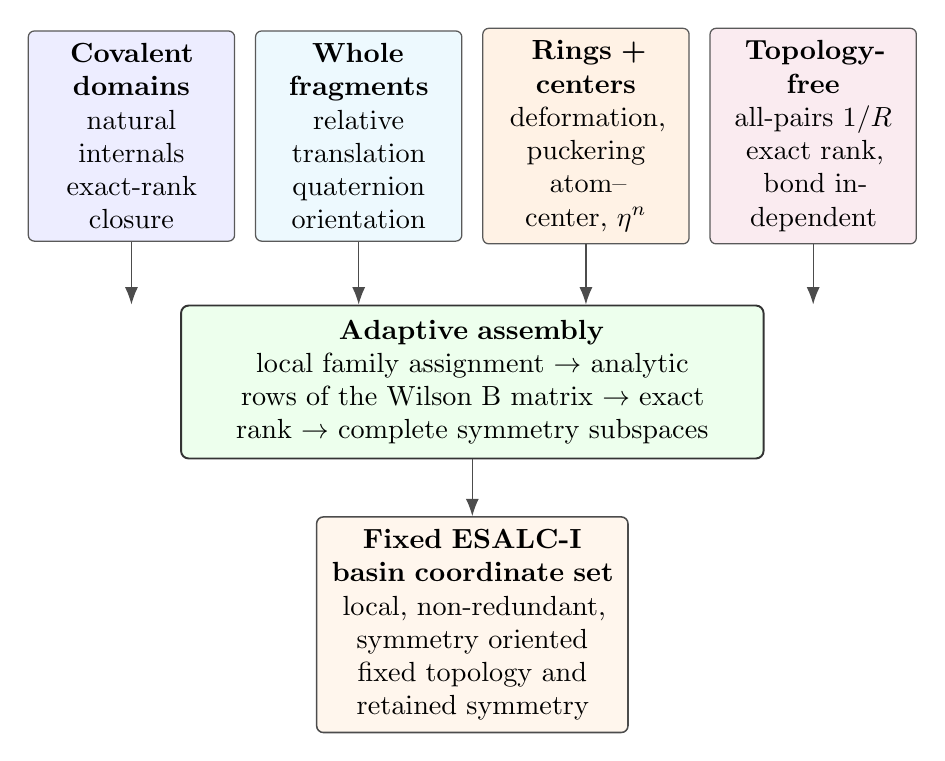
\begin{tikzpicture}[
  node distance=0.55cm and 0.25cm,
  every node/.style={font=\normalsize},
  domainbox/.style={
    draw=black!65,
    line width=0.45pt,
    rounded corners=2.2pt,
    align=center,
    text width=0.19\linewidth,
    minimum height=1.24cm,
    inner sep=4.5pt,
    fill=#1
  },
  core/.style={
    draw=black!80,
    line width=0.70pt,
    rounded corners=2.8pt,
    align=center,
    text width=0.58\linewidth,
    minimum height=1.18cm,
    inner sep=5.2pt,
    fill=green!7
  },
  output/.style={
    draw=black!70,
    line width=0.55pt,
    rounded corners=2.4pt,
    align=center,
    text width=0.30\linewidth,
    minimum height=1.08cm,
    inner sep=4.5pt
  },
  arrow/.style={-{Latex[length=2.2mm]}, line width=0.45pt, draw=black!70}
]
\node[domainbox=blue!7] (covalent) {\textbf{Covalent domains}\\natural internals\\exact-rank closure};
\node[domainbox=cyan!7, right=of covalent] (fragments) {\textbf{Whole fragments}\\relative translation\\quaternion orientation};
\node[domainbox=orange!10, right=of fragments] (centers) {\textbf{Rings + centers}\\deformation, puckering\\atom--center, \(\eta^n\)};
\node[domainbox=purple!8, right=of centers] (coordination) {\textbf{Topology-free}\\all-pairs \(1/R\)\\exact rank, bond independent};

\node[core, below=0.78cm of $(fragments.south)!0.5!(centers.south)$] (assembly)
  {\textbf{Adaptive assembly}\\local family assignment \(\rightarrow\) analytic {rows of the Wilson B matrix}
   \(\rightarrow\) exact rank \(\rightarrow\) complete symmetry subspaces};

\node[output, fill=orange!7, below=0.72cm of assembly] (sonic)
  {\textbf{{Fixed ESALC-I basin coordinate set}}\\local, non-redundant, symmetry oriented\\fixed topology and retained symmetry};

\foreach \source in {covalent,fragments,centers,coordination}
  \draw[arrow] (\source.south) -- (\source.south |- assembly.north);
\draw[arrow] (assembly.south) -- (sonic.north);
\end{tikzpicture}
}
\caption{{Construction of a fixed ESALC-I coordinate set from
chemically perceived domains, local families, rank reduction, and the retained
molecular symmetry.}}
\label{fig:construction-sequence}
\end{figure}

{Every retained coordinate remains linked to its defining
local motion. Figure~\ref{fig:coordinate-atlas} illustrates a ring-puckering
combination of four single-atom out-of-plane (SOOP) source functions. Their
values are denoted by \(s_1,\ldots,s_4\); their coefficients define one local
coordinate. The illustrative label \(\mathrm{RPck001}\) identifies that
ring-puckering combination. Its chemical family, molecular-symmetry label,
and analytic Wilson B matrix row accompany the definition. The arrows show
the corresponding infinitesimal Cartesian motion; the displayed
\(-h,0,+h\) views illustrate this direction, not an optimization path.}

\begin{figure}[htbp]
\centering
\includegraphics[width=\linewidth]{figures/sonic_coordinate_atlas.pdf}
\caption{{Schematic ring-puckering coordinate assembled
from SOOP sources, with its coefficients, symmetry, and analytic Wilson B
matrix row. Arrows show an infinitesimal displacement.}}
\label{fig:coordinate-atlas}
\end{figure}

{The following sections describe the construction and test its rank,
locality, symmetry, and use in geometry optimization.}

\section{Coordinate Construction: From Structural Primitives to a Fixed {Coordinate Basis}}

{Construction begins with a molecular state and a deliberately
redundant pool of typed primitive functions.  Each function has a chemical
domain and family; local combinations are formed within those assignments.
Selection of independent Wilson B matrix rows closes the physical internal
space, and molecular-symmetry projection orients each family without erasing
its assignment.  Figure~\ref{fig:construction-sequence} gives this order; the following
subsections define its inputs, domain rules, and rank and symmetry operations.}

{Let \(T\) denote the tangent space of overall translations and rotations.
An independent basis for an \(N\)-atom structure has \(3N-\dim T\)
directions. The local relation between Cartesian coordinates \(\x\) and
internal coordinates \(\q\) is}
{
\begin{equation}
\begin{split}
  \Delta q_i
  &=q_i(\x+\Delta\x)-q_i(\x) \\
  &=\sum_{a=1}^{3N} B_{ia}\Delta x_a
   +\frac{1}{2}\sum_{a,b=1}^{3N} C_{iab}\Delta x_a\Delta x_b
   +\mathcal{O}(\lVert\Delta\x\rVert^3),
\end{split}
  \label{eq:wilson-intro}
\end{equation}
}
{Here \(B_{ia}=\partial q_i/\partial x_a\) and
\(C_{iab}=\partial^2q_i/(\partial x_a\partial x_b)\).  The Wilson B matrix
gives the tangent map \(\Delta\q=\Bmat\Delta\x\) to first order;
coordinate construction supplies its chemically meaningful independent
rows.\cite{Wilson1955}  Higher derivatives describe coordinate curvature.}

{The same distinction appears in the Hessian.  For a local
Cartesian realization \(\x(\q)\), with
\(\Jmat=\partial\x/\partial\q\),}
{
\begin{equation}
 \nabla_{\!\q}^{2}E
 =\Jmat^{\mathsf T}\nabla_{\!\x}^{2}E\,\Jmat
 +\sum_{a=1}^{3N}\frac{\partial E}{\partial x_a}
   \nabla_{\!\q}^{2}x_a .
 \label{eq:asymptotic-hessian}
\end{equation}
}
{At a stationary point the Cartesian gradient vanishes. We implement the
Hessian transformation on the vibrational tangent space as
\(\nabla_{\!\q}^{2}E=(\Bmat^+)^{\mathsf T}\nabla_{\!\x}^{2}E\,\Bmat^+\),
where \(\Bmat^+\) is the inverse (for non-redundant sets) or pseudoinverse (for redundant sets) of the Wilson B matrix. Thus only
\(\Bmat\), rather than second derivatives of the coordinates, is needed.
Exact rank preserves the physical quadratic model there; locality and
complete symmetry blocks determine how clearly that model can be inspected
and approximated before convergence. The construction is therefore judged
by rank, chemical content, and symmetry as separate properties.}

\subsection{Primitive Sources and the Molecular State}

{The construction starts from primitive coordinate functions,
not from a preselected numerical basis.  Within a basin, topology, primitive
identities, and the selected molecular symmetry remain fixed. At its entry,
chemical perception specifies covalent and multicenter
connectivity, coordination environments, fragment partition, ring decomposition,
pseudobonds and structural interaction centers. Primitive identities and
their family assignment are then fixed for that basin. At a boundary, changes
in topology, primitive assignments, or selected symmetry are identified before a new
non-redundant basis is formed.  If the primitive assignment is uncertain,
{we construct the complete, non-redundant ESALC-C basis from
Cartesian directions after removing overall translations and rotations,
without requiring a bond assignment.}  The perception criteria and
reassessment thresholds follow the published perception method\cite{Barone2026Perception}
and are implemented in the coordinate-construction code.}

The primitive layer is deliberately redundant.  It includes one distance for
each covalent edge, angular sources around bonded centers, the two transverse
components required at linear centers, candidate dihedrals about eligible
bonds, and single-atom out-of-plane sources at three-coordinate centers.
Rings contribute endocyclic angles and ring-owned single-atom out-of-plane
sources, including at tetracoordinate atoms. Fragment translations and
orientations, atom--center functions, multicenter bridges, and all-pairs
inverse distances supply sources for their respective domains.  Redundancy is useful
at this stage because every plausible local motion can be generated before
linear dependence is removed.  Each source is assigned both a physical family
and a structural domain, and these assignments remain attached to every
combination formed from it.

Let \(\mathbf p\) collect the ordered source functions and let \(\mathbf C\)
contain the coefficients of the retained combinations.  The active
coordinates and their {Wilson B matrix} are
\begin{equation}
  \q=\mathbf C\mathbf p,
  \qquad
  \Bmat_{\q}=\mathbf C\Bmat_{\mathbf p}.
  \label{eq:source-to-active}
\end{equation}
The source pool may be overcomplete, whereas the rows of
\(\Bmat_{\q}\) always form a non-redundant internal basis.  Rank-neutral
variables \(\y=f(\q)\), including proton-transfer combinations,
trigonometric torsions, and Cremer--Pople amplitudes and phases, are evaluated
from that basis by the chain rule and do not add directions to it.

{For each retained coordinate, its definition gives the source functions, combination
coefficients, chemical family, symmetry label, and Wilson B matrix row.  The optimizer receives the complete set of coordinate
definitions.  Figure~\ref{fig:coordinate-atlas} illustrates one row; the
numerical details are given in SI Sec.~S2.}

\subsection{Recognition of Structural Domains and Construction Sequence}

The molecular graph is examined recursively before generic angle and torsion
lists are completed.  The sequence follows the chemically successful logic of
generalized natural internal coordinates: terminal groups are resolved first,
followed by isolated rings, spiro rings, and fused rings, and the
search is repeated because removing a completed environment can expose the
next one.\cite{VonArnimAhlrichs1999GNIC}  Here the same recursion is expressed
through assignment of primitive source functions to chemical domains.  A recognized domain remains an explicit
block, so the procedure also accommodates overlapping fused and bridged rings,
cages, locally symmetric coordination spheres, persistent fragments,
multicenter bridges, and haptic or center-based interactions.

The complete sequence is as follows.  Covalent stretches first establish the
bonded frame.  Recursive graph analysis then identifies terminal groups and
the isolated, spiro, fused, bridged, and cage ring domains.  Ring perception
supplies canonical cyclic orders, joins cycles that share vertices, edges, or
paths, and assigns every shared source only once.\cite{Downs1989RingPerception,Lee2009RingPerception,MaySteinbeck2014Rings}  The unresolved bonded
centers then supply ordinary or linear bends, while graph environment, ligand
identity, and geometry identify local rotors and high-coordination patterns.
Fragment, multicenter, and interaction-center domains are added before the
remaining valence space is filled.  Finally, ordinary exocyclic torsions and
other residual coordinates complete the source space.  A primitive already
owned by a completed domain is excluded from generic completion, preventing
the same physical motion from being represented twice under different names.

This order converts each recognized structural element into a complete family
before rank reduction.  Ring deformation therefore remains distinct from
puckering and butterfly motion; relative fragment orientation remains distinct
from intrafragment deformation; and stretches, angles, and torsions are not
mixed simply because they span the same tangent space.  Delocalization is
confined to a homogeneous family or to the residual space for which no more
specific chemical construction is available.  The subsequent molecular
symmetry adaptation is likewise performed separately within each family.

\subsection{Coordinate Families}

The atlas of coordinate families is open-ended.
The candidate coordinates are assembled in a fixed chemical order.  All covalent
{stretches} are generated first.  Exocyclic valence angles are organized as
local symmetry-adapted combinations around each center, with explicit
templates from \(XY_2\) and \(XY_3\) through the qualified coordination
geometries up to coordination number (CN) 14.\cite{ZouTaoKraka2020Polytopal}  Exocyclic dihedrals follow, one representative per
eligible bond, selected by Prelog ordering and, for ties, by effective nuclear
charge and local connectivity; every three-coordinate center contributes its
complete oriented out-of-plane family.  Cyclic valence angles and endocyclic
dihedrals are then built from the regularized ring source space, retaining
butterfly rows for collective folds.  Fragment pose, atom--center, \(\eta^n\), multicenter, and
topology-independent families complete the typed source pool.  Only after this
construction are the rows reduced by singular-value/rank tests, completed
across families by retaining only independent rows needed to close rank, and
symmetry-oriented within each family.

{The algebraic order is primitive generation, chemically local
symmetry-adapted linear combinations, singular-value analysis of the resulting
Wilson B matrix, and final molecular-symmetry orientation within each family.
Alternative admissible primitive selections and independent ESALC-I combinations
are compared by the condition number
\(\kappa_2(\widetilde{\Bmat})=\sigma_{\max}/\sigma_{\min}^{+}\),
where each nonzero row is normalized as
\(\widetilde{\Bmat}_{i:}=\Bmat_{i:}/\|\Bmat_{i:}\|_2\),
\(\sigma_{\max}\) is the largest singular value of \(\widetilde{\Bmat}\),
and \(\sigma_{\min}^{+}\) is its smallest retained nonzero singular value.
The selected primitive set and coordinate dimensions remain fixed within the
basin.}

The coordinate families are summarized in Table~\ref{tab:coordinate-types}.
Its breadth is essential: no single conventional family describes with equal
clarity a covalent chain, a fused ring, a weak complex, and a highly
coordinated cluster.  Automatic domain assignment chooses among these families,
and exact-rank selection then joins them into one basis.

\begin{table}[htbp]
\centering
\scriptsize
\setlength{\tabcolsep}{3pt}
\caption{Coordinate families used in the automatic construction.}
\label{tab:coordinate-types}
\begin{tabularx}{\linewidth}{@{}>{\raggedright\arraybackslash}p{0.20\linewidth}
>{\raggedright\arraybackslash}p{0.34\linewidth}
>{\raggedright\arraybackslash}X@{}}
\toprule
Family & Representative coordinates & Physical role \\
\midrule
Covalent domains & All stretches; ordinary or linear bend; exocyclic torsion;
complete tricoordinate out-of-plane family & Canonical local valence source
space and ordinary residual completion. \\
\midrule
Locally symmetric domains & \(XY_3/XY_2\) symmetry-adapted linear combinations
(SALCs); collective rotors;
high-coordination templates & Chemically qualified sums, differences, rocks,
and deformations within one homogeneous family. \\
\midrule
Ring domains & Ring deformation; regularized endocyclic angles;
aromatic/non-aromatic dihedrals; linear Cartesian SOOP combinations with
geometry-updated coefficients and fixed coordinate identities; minimal signed puckering;
butterfly and collective inter-ring motion & Complete fused, bridged, spiro,
and cage source spaces claimed before generic torsions. \\
\midrule
Multicenter domains & Shared N/O/P/S proton; electron-deficient H/halogen
bridges at B, Al and related centers; O--O, O--S, S--S, S--Se and Se--Se
closures; metal--ligand, structural-center and \(\eta^n\) distance/orientation & Multicenter,
cyclic, electron-deficient, or haptic chemistry represented directly as primary
domains. \\
\midrule
Interfragment blocks & Relative translations; exponential-map orientations;
open-contact pseudobonds; closed-graph exponential-map pose & Relative fragment
motion and basin-specific contact interfaces, with typed contact--pose
completion when required. \\
\midrule
Topology-independent domains & All-pairs inverse distances; ESALC-C when required & Bond-independent description of
molecules with ambiguous topology or highly coordinated domains. \\
\midrule
Derived variables & Inverse/exponential distances; trigonometric torsions;
proton-transfer functions; Cremer--Pople amplitudes/phases & Functions that can
make the local potential-energy surface more nearly quadratic without changing
the rank of the non-redundant basis. \\
\bottomrule
\end{tabularx}
\end{table}

{
\begin{center}
\resizebox{0.98\linewidth}{!}{%
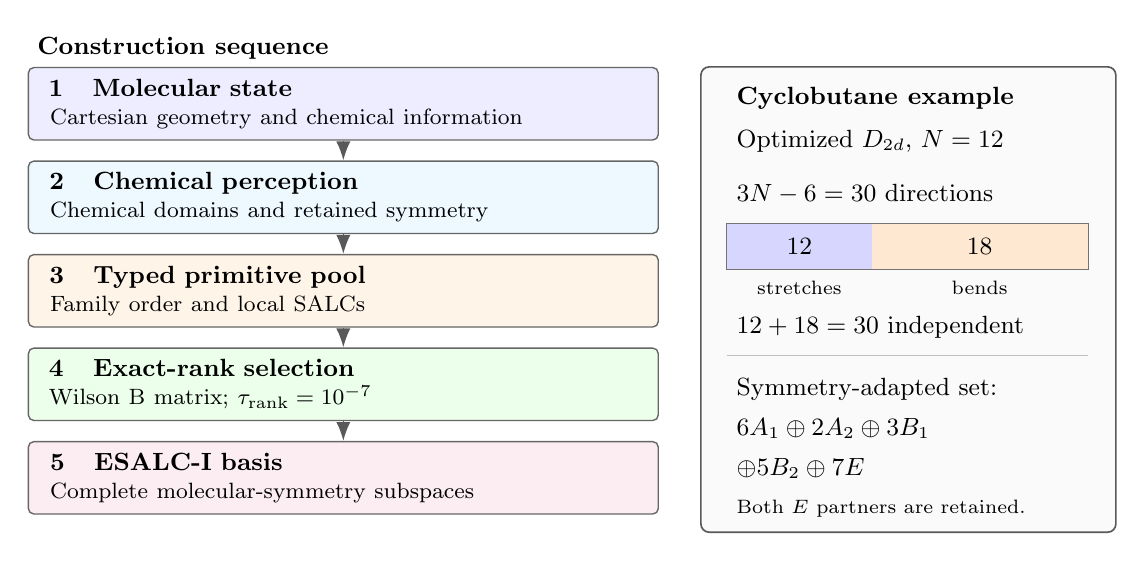
\begin{tikzpicture}[
  flowbox/.style={draw=black!60, rounded corners=2pt, line width=0.5pt,
    minimum width=8.0cm, minimum height=0.92cm, align=left,
    text width=7.45cm, inner xsep=0.26cm, font=\small},
  flow/.style={-{Latex[length=2.4mm]}, draw=black!65, line width=0.6pt}
]
\node[font=\bfseries\small, anchor=west] at (0,6.72) {Construction sequence};
\node[flowbox, fill=blue!7, anchor=north west] (state) at (0,6.48)
  {\textbf{1\quad Molecular state}\\[-1pt]
   {\footnotesize Cartesian geometry and chemical information}};
\node[flowbox, fill=cyan!7, below=0.25cm of state] (perception)
  {\textbf{2\quad Chemical perception}\\[-1pt]
   {\footnotesize Chemical domains and retained symmetry}};
\node[flowbox, fill=orange!9, below=0.25cm of perception] (families)
  {\textbf{3\quad Typed primitive pool}\\[-1pt]
   {\footnotesize Family order and local SALCs}};
\node[flowbox, fill=green!8, below=0.25cm of families] (rank)
  {\textbf{4\quad Exact-rank selection}\\[-1pt]
   {\footnotesize Wilson B matrix; \(\tau_{\mathrm{rank}}=10^{-7}\)}};
\node[flowbox, fill=purple!7, below=0.25cm of rank] (symmetry)
  {\textbf{5\quad ESALC-I basis}\\[-1pt]
   {\footnotesize Complete molecular-symmetry subspaces}};
\foreach \a/\b in {state/perception,perception/families,families/rank,rank/symmetry}
  \draw[flow] (\a.south) -- (\b.north);

\draw[black!65, rounded corners=3pt, line width=0.6pt, fill=black!2]
  (8.55,0.57) rectangle (13.82,6.48);
\node[font=\bfseries\small, anchor=west] at (8.88,6.08)
  {Cyclobutane example};
\node[font=\small, anchor=west] at (8.88,5.53)
  {Optimized \(D_{2d}\), \(N=12\)};
\node[font=\small, anchor=west] at (8.88,4.87)
  {\(3N-6=30\) directions};
\fill[blue!16] (8.88,3.91) rectangle (10.72,4.49);
\fill[orange!18] (10.72,3.91) rectangle (13.47,4.49);
\draw[black!55] (8.88,3.91) rectangle (13.47,4.49);
\node[font=\small] at (9.80,4.20) {12};
\node[font=\small] at (12.09,4.20) {18};
\node[font=\scriptsize] at (9.80,3.67) {stretches};
\node[font=\scriptsize] at (12.09,3.67) {bends};
\node[font=\small, anchor=west] at (8.88,3.17)
  {\(12+18=30\) independent};
\draw[black!25] (8.88,2.81) -- (13.47,2.81);
\node[font=\small, anchor=west] at (8.88,2.39)
  {Symmetry-adapted set:};
\node[font=\small, anchor=west] at (8.88,1.89)
  {\(6A_1\oplus2A_2\oplus3B_1\)};
\node[font=\small, anchor=west] at (8.88,1.38)
  {\(\oplus5B_2\oplus7E\)};
\node[font=\scriptsize, anchor=west] at (8.88,0.87)
  {Both \(E\) partners are retained.};
\end{tikzpicture}%
}
\end{center}
}

{Figure~\ref{fig:coordinate-family-atlas} shows how the typed
sources retain their chemical identity through rank reduction and symmetry
orientation.}

\begin{figure}[htbp]
\centering
\includegraphics[width=0.98\linewidth]{figures/coordinate_family_atlas.pdf}
\caption{{Coordinate-family atlas showing typed sources and
their symmetry-oriented blocks.}}
\label{fig:coordinate-family-atlas}
\end{figure}

\subsubsection{Local covalent and symmetry-adapted families}
\label{sec:local-pseudosymmetry}

{Covalent domains begin with one stretch per bond, angular sources at bonded
centers, and two transverse bending components where an ordinary angle
becomes singular at linearity. Chemically equivalent ligands form a local
orbit only when their connectivity, continuous descriptors, and geometry
support the assignment. Within that orbit, a totally symmetric sum and its
orthonormal complements form local SALCs. These combinations describe
recognizable stretching, bending, rocking, and out-of-plane motions even
when the full molecule has little symmetry; exact molecular irreducible
representations are assigned only at the final projection.}

{As an example, Figure~\ref{fig:capped-octahedron-salcs} identifies all seven metal--ligand
stretches in a capped-octahedral coordination sphere of local \(C_{3v}\)
symmetry. With central atom \(M\) and ligands \(L_1,\ldots,L_7\),
\(r_i=|\mathbf R_{L_i}-\mathbf R_M|\): \(r_1\) joins the cap, \(r_2,r_3,r_4\)
join the capped face, and \(r_5,r_6,r_7\) join the opposite face. The two
face triplets remain separate local orbits.}

\begin{figure}[htbp]
\centering
\input{figures/capped_octahedron_salc.tex}
\caption{Schematic projection of seven metal--ligand stretches at a capped-octahedral center.
Dashed triangles identify the two three-ligand orbits.}
\label{fig:capped-octahedron-salcs}
\end{figure}

{The cap stretch \(r_1\) is totally symmetric. For each face triplet
\(\mathbf q=(q_1,q_2,q_3)=(r_2,r_3,r_4)\) or \((r_5,r_6,r_7)\), the local
SALCs are}
\begin{equation}
\begin{aligned}
 S_{A_1}(\mathbf q)&=(q_1+q_2+q_3)/\sqrt{3},\\
 S_{E,1}(\mathbf q)&=(2q_1-q_2-q_3)/\sqrt{6},\\
 S_{E,2}(\mathbf q)&=(q_2-q_3)/\sqrt{2}.
\end{aligned}
\label{eq:capped-octahedral-salcs}
\end{equation}
\begin{samepage}
{Together with the cap stretch, the two triplets give seven stretching
directions of local symmetry \(3A_1+2E\). The valence angles
\(\theta_{ij}=\angle L_iML_j\) likewise form local symmetry orbits. For the
eight atoms in Fig.~\ref{fig:capped-octahedron-salcs}, define the four
three-angle orbits and the two halves of the six-angle cross-face orbit as}
\begin{equation}
\begin{aligned}
\mathbf t&=(\theta_{12},\theta_{13},\theta_{14}), &
\mathbf u&=(\theta_{15},\theta_{16},\theta_{17}),\\
\mathbf v&=(\theta_{34},\theta_{24},\theta_{23}), &
\mathbf w&=(\theta_{67},\theta_{57},\theta_{56}),\\
\mathbf a&=(\theta_{26},\theta_{37},\theta_{45}), &
\mathbf b&=(\theta_{27},\theta_{35},\theta_{46}).
\end{aligned}
\label{eq:capped-octahedral-angle-orbits}
\end{equation}
{Using the triplet combinations of Eq.~\ref{eq:capped-octahedral-salcs},
one explicit independent angular set is}
\begin{equation}
\begin{aligned}
\mathcal S_{\mathrm{cap}}={}&\{S_{A_1}(\mathbf t),S_{E,1}(\mathbf t),S_{E,2}(\mathbf t),
S_{A_1}(\mathbf u),S_{E,1}(\mathbf u),S_{E,2}(\mathbf u)\},\\
\mathcal S_{\mathrm{face}}={}&\{S_{E,1}(\mathbf v),S_{E,2}(\mathbf v),
S_{E,1}(\mathbf w),S_{E,2}(\mathbf w)\},\\
S_{A_2}^{\times}={}&(a_1+a_2+a_3-b_1-b_2-b_3)/\sqrt{6}.
\end{aligned}
\label{eq:capped-octahedral-angular-salcs}
\end{equation}
{These six cap-related rows, four face rows, and one cross-face row span
the 11 angular directions with local symmetry \(2A_1+A_2+4E\). The
opposite-ligand angles \(\theta_{25},\theta_{36},\theta_{47}\) equal
\(180^\circ\) in the ideal octahedral core and are excluded as singular
ordinary-angle sources; the other angle orbits already close the angular
rank. Thus the seven stretches and 11 angular directions close the rank-18
internal space. No dihedral is needed for this bare coordination sphere.
Familywise rank selection and final molecular-symmetry projection then act
on every accepted family.}
\end{samepage}

{An ordinary exocyclic bond contributes one deterministically chosen physical
dihedral. A collective rotor is used when its complete local domain and
reference direction are recognized. If a proposed local pattern is not
supported, ordinary coordinates fill the same physical space under the
unchanged rank criterion. Each accepted coordinate retains its chemical
family in the final basis.}

\subsubsection{Rings, puckering, and collective deformation}
\label{sec:ring-coordinates}

{Each ring is treated as a domain before generic torsions are generated.
Endocyclic valence angles describe ring deformation. Ring-owned
single-atom out-of-plane sources supply puckering directions from the
endocyclic bonds, including at tetracoordinate ring atoms. Such atoms have no
separate local umbrella coordinate: valence angles span their other angular
motions. Independent combinations yield the \(n-3\) puckering directions
of an isolated \(n\)-membered ring, with derivatives finite at planarity. Cremer--Pople amplitudes and phases describe
ring shape as functions of the selected basis and add no rank-carrying
directions.\cite{CremerPople1975,RingPuckering2021,LemaSaavedraFernandezRamos2026RingCP}}

{Fused, spiro, bridged, and cage rings are assembled as connected source
spaces. Shared sources are counted once, and explicit butterfly rows describe
collective folds. Ring deformation, puckering, and inter-ring motion retain
separate family identities through exact-rank selection and molecular
symmetry projection.}

This compact set of coordinate families is complementary: local covalent
coordinates describe ordinary bonding, collective families describe rings and
symmetry-related sites, and the remaining sections extend the same construction
to topology-independent domains, fragment pose, and multicenter interactions.
\subsection{Topology-independent and fragment coordinates}

Topology-independent domains use the non-null space of all pairwise inverse
distances.\cite{BakerPulay1996Inverse,Maslen2005Scaled}  This representation supplies a continuous {coordinate basis} when a covalent
graph is unavailable or changing, while the physical (1/R) limit is retained
at fragment separation.  Exact-rank selection determines the usable subspace
before symmetry orientation.

Persistent fragments are described by relative translations and orientations,
with intrafragment deformation kept distinct from rigid-body motion.\cite{BakerPulay2000Clusters,Krautgasser2016Surface}  Open
contacts use dedicated interaction coordinates; closed contacts use the
corresponding relative-pose description.  Multicenter and haptic interactions
are represented by structural centers and typed local families.  These choices
preserve fragment identity and avoid introducing artificial covalent bonds.

The same domain-first policy covers weak complexes, chemisorption, and
high-coordination structures. Each physical domain receives its coordinates
before the final basis is assembled. The SI gives the contact rules, pose
functions, multicenter constructions, and representative rank audits.

{Figure~\ref{fig:adsorption-coordinate-atlas} illustrates this
selection for four model NH$_3$ adsorption environments. Water networks,
fused rings, and cages admit chemically assigned ESALC-I families; a metal
cluster may instead use independent all-pairs inverse-distance directions.
The interface receives fragment-pose or typed contact coordinates. If the
primitive assignment becomes ambiguous, the entire molecular system uses
ESALC-C.}

\begin{figure}[htbp]
\centering
\includegraphics[width=\linewidth]{figures/chemisorption_block_partition.pdf}
\caption{{Examples of coordinate selection for NH$_3$
adsorption environments. Ambiguous assignments invoke full-system ESALC-C.}}
\label{fig:adsorption-coordinate-atlas}
\end{figure}

{Structural centers provide reference points without adding
fictitious atoms. A center--atom distance differentiates through the atoms
that define its center. Figure~\ref{fig:special-coordinate-structures}
illustrates ring centers in ferrocene, a supplied $\eta^3$ ligand center,
weak contacts, and relative fragment pose. Their analytic derivatives and
rank contributions are treated by the same Wilson B matrix audit as ordinary
coordinates.}

\begin{figure}[htbp]
\centering
\includegraphics[width=\linewidth]{figures/special_coordinate_structures.png}
\caption{{Special-coordinate examples: structural centers,
weak contacts, and relative fragment pose.}}
\label{fig:special-coordinate-structures}
\end{figure}

{ESALC-C uses Cartesian displacement directions projected
orthogonally to \(T\), leaving a complete independent vibrational basis.
The remaining space is oriented in
complete molecular-symmetry subspaces, so it retains the physical rank and
the molecular point group without a bond assignment. ESALC-C therefore
supplies a complete alternative representation when chemically assigned
primitive functions cease to be reliable.}
\subsection{Exact-rank selection across families}

{Rank selection receives the ordered primitive functions,
their analytic Wilson B matrix rows, and their chemical-family assignments.
Complete ring, fragment, interaction-center, and other specialized domains
are considered before ordinary completion candidates. Each family contributes
only the part independent of the previously accepted rows; a dependent
torsion, for example, cannot turn into a stretch--bend--torsion combination.
For a candidate row \(\mathbf b_i\), the row-normalized residual against the
accepted orthonormal span \(\{\widehat{\mathbf b}_j\}\) is}
{
\begin{equation}
 \rho_i=\left\|
 \frac{\mathbf b_i}{\|\mathbf b_i\|_2}
 -\sum_{j\in A}
 \left(\frac{\mathbf b_i}{\|\mathbf b_i\|_2}\cdot
 \widehat{\mathbf b}_j\right)\widehat{\mathbf b}_j
 \right\|_2 .
 \label{eq:rank-residual}
\end{equation}
}
{The candidate is retained when
\(\rho_i>\tau_{\mathrm{rank}}=10^{-7}\). Rank-revealing
orthogonal--triangular (QR) factorization or a thin singular-value
decomposition resolves dependent rows within a family;\cite{GolubReinsch1970} the final audit
closes the rank across families. Normalization prevents the different units
of stretches, angles, and fragment motions from deciding the rank. SI
Secs.~S2.8 and S2.11--S2.13 give the numerical procedure and its formal
properties.}

The final audit verifies the physical rank; a rank defect identifies an
incomplete candidate set.
{Within one basin, a nonzero selection margin preserves the
accepted primitive identities and family dimensions under small geometric
changes.  If ESALC-I becomes poorly conditioned, loses rank, or its primitive
assignment becomes ambiguous, chemical perception is repeated and the
optimization proceeds with a complete, symmetry-adapted ESALC-C basis for the
whole molecule.  Where a stable primitive assignment is available at the
converged geometry, one optional final ESALC-I iteration can express and refine
that endpoint in chemically interpretable coordinates.  A regional mixed
ESALC-I/ESALC-C implementation exists but is not used in the calculations
reported here.}
\subsection{Intrafamily molecular symmetry}

{Exact rank determines how many coordinates are needed; molecular symmetry
determines how those coordinates are organized. Local SALCs reflect chemical
equivalence within a domain, whereas the final point-group operations assign
exact molecular irreducible representations. For each family closed under
those operations, the character projector selects the complete subspace of
irrep \(\alpha\):}
{
\begin{equation}
 \Pi_\alpha^{(F)}=
 \frac{\ell_\alpha}{|G|}
 \sum_{g\in G}\chi_\alpha(g)^*\,\Gamma_F(g),
 \label{eq:family-symmetry-projector}
\end{equation}
}
{Here \(\ell_\alpha\) and \(\chi_\alpha\) are its dimension and character,
and \(\Gamma_F\) is the operation on family \(F\). Every partner of a
multidimensional irrep is retained. Sharing an irrep never causes a stretch
and a torsion to be mixed.}

{A final Wilson B matrix rank audit checks the projected
families together. If individually valid family choices are collectively
dependent, combinations are exchanged within their families while their
assigned dimensions are preserved. An incompatible assignment is reported.
The full basis remains available for structural analysis, while an optimizer
may activate its totally symmetric subset. SI Sec.~S2 gives the projectors,
phase conventions, and non-Abelian examples.}
\section{Validation}
\label{sec:validation}

\subsection{Construction Checks and Stability}
\label{sec:construction-stability}

{We test the coordinate sets at three levels.  First, rank
and analytic-derivative checks establish that the assigned families span the
physical internal space.  Second, a common Cartesian Hessian tests the
locality and symmetry of the resulting representation.  Finally, fixed
coordinate sets are supplied to geometry optimizers.  Gaussian's
\texttt{ReadAllGIC} input reads the generated coordinates in the
paired Gaussian tests.\cite{GaussianGICManual} SI Sec.~S3 specifies the
Gaussian input; the remaining SI sections give protocols and numerical tables.}

{Figure~\ref{fig:validation-molecules} identifies structures
chosen to expose distinct construction demands: bridged rings,
fragment pose, interaction centers, and a puckering path.  We report larger
molecules separately as construction and optimization checks at approximately
100 atoms.}

\begin{figure}[H]
\centering
\includegraphics[width=0.95\linewidth]{figures/validation_molecule_panel.pdf}
\caption{Validation systems spanning bridged rings, centers, fragment pose,
and an $\eta^3$ ligand; the cyclohexane panels show the chair--boat path.}
\label{fig:validation-molecules}
\end{figure}

{Figure~\ref{fig:large-molecule-validation} shows the
78--113-atom structures used for a size check: an extended porphyrin and
two flexible taxanes generated from molecular graphs.  Their coordinate
bases were first audited for rank, sparsity, and conditioning, then supplied
to Gaussian for separate Parametrized Model 6 (PM6) optimization checks.\cite{Stewart2007PM6}}

\begin{figure}[htbp]
\centering
\includegraphics[width=\linewidth]{figures/large_molecule_validation_panel.png}
\caption{{Large-molecule construction tests:
tetraphenylporphyrin (78 atoms), docetaxel (111 atoms), and paclitaxel
(113 atoms).}}
\label{fig:large-molecule-validation}
\end{figure}

{We assess conditioning from the nonzero singular values of the
Wilson B matrix after normalizing each nonzero row to unit Euclidean norm.
All three coordinate bases closed exactly at the internal dimension, with ranks
228/228, 327/327, and 333/333.  Their Wilson B matrices had nonzero
fractions of 9.2, 4.7, and 4.8\%, respectively.  These
results are construction checks on graph-derived three-dimensional structures;}
SI Sec.~S4 reports separate reference-path construction measurements and the
hardware details for the optimization tests.

{Figure~\ref{fig:construction-cost} plots construction time,
one analytic Wilson B matrix evaluation, and peak Python allocation for 13
systems of 12--36 atoms, including polycyclic aromatic hydrocarbons (PAHs).
Ferrocene has the largest candidate pools
(651--656) and measured costs. Construction combines family assembly, rank
reduction, symmetry orientation, and output. The measured range and numerical
data are given in SI Sec.~S4.}

\begin{figure}[htbp]
\centering
\includegraphics[width=\linewidth]{figures/construction_cost.pdf}
\caption{{Construction time, one analytic Wilson B matrix
evaluation, and peak Python allocation for 13 systems. Medians of five
single-process runs on dual AMD EPYC 7543 processors (Linux x86-64).}}
\label{fig:construction-cost}
\end{figure}

As a computational check on this size range, the tetraphenylporphyrin,
docetaxel, and paclitaxel {coordinate bases} were used by Gaussian with the
semiempirical PM6 method and compared
with Gaussian's native internal-coordinate route at the same PM6 level.  All
three ESALC-I paths reached normal termination in 17, 116, and 72 optimization
steps, respectively.  These PM6 runs extend the controlled comparison to
medium-to-large structures.  The construction check and its
timings, reported in SI Sec.~S4, remain independent of the electronic-structure
method.

{Table~\ref{tab:validation} gives representative
construction checks across rings, cages, weak complexes, and an interaction
center; SI Sec.~S5 reports the full set.  Rank/target tests completeness.
For nontrivial local combinations,
\(\epsilon_{\mathrm{SALC}}=\max_i|\sum_j c_{ij}^{2}-1|\) measures
normalization error; the finite-difference (FD) error \(\epsilon_{\mathrm{FD}}\)
is the maximum difference between analytic and numerical Wilson B matrix
elements.  Every
listed system reaches its target rank while retaining the coordinate families
appropriate to its structure. The complete norbornane construction example
and its Gaussian-readable coordinate input appear in SI Listings S1 and S2.}
\begin{table}[htbp]
\centering
\footnotesize
\setlength{\tabcolsep}{4pt}
\caption{{Representative rank, symmetry, and derivative checks
for coordinate construction.}}
\label{tab:validation}
\begin{tabularx}{\linewidth}{@{}l>{\raggedright\arraybackslash}Xc l>{\raggedright\arraybackslash}X@{}}
\toprule
System & Structural feature & {Point group} & Rank/closure & Validation result \\
\midrule
Azulene & Non-benzenoid fused ring; butterfly & \(C_{2v}\) & 48/48; six puckering rows & \(\epsilon_\mathrm{SALC}=2.22\times10^{-16}\) \\
Norbornane & Bridged saturated ring & \(C_{2v}\) & 51/51; three puckering rows & \(\epsilon_\mathrm{SALC}=2.22\times10^{-16}\) \\
Cubane & High-symmetry cage & \(O_h\) & 42/42; cyclic bends & \(\epsilon_\mathrm{SALC}=2.22\times10^{-16}\) \\
Indane & Fused aromatic/alicyclic rings & \(C_s\) & 51/51 & \(\epsilon_\mathrm{FD}=4.77\times10^{-10}\); butterfly and puckering rows \\
Saccharin & Fused heterocycle; butterfly--puckering & \(C_s\) & 45/45; five puckering rows & \(\epsilon_\mathrm{FD}=3.91\times10^{-10}\); post-projector rank 45 \\
Formic acid--water & Weak-complex fragment pose & \(C_1\) & 18/18; 6 interfragment & three translations and three orientations; direct \(\Bmat\)-rank 18 \\
$\eta^3$ allyl--PdCl & $\eta^3$ ligand center & \(C_1\) & 24/24; center row & \(q_{\eta^3}=1.8000\)~\AA; analytic center--atom row retained \\
\bottomrule
\end{tabularx}
\end{table}

Near-planar fused rings are described by signed curvilinear flap and butterfly
rows with finite Wilson derivatives at planarity.  Indane verifies their
finite-difference accuracy, while saccharin probes the coupled case in which
one butterfly and five puckering rows share \(A''\) symmetry.  Intrafamily
projection on the physical Wilson-row spaces preserves all 45 coordinates and
selects the independent inter-ring motion.

Complete finite-difference tests on all 114 pagodane and 51 indane coordinates
confirm the accuracy of the analytic chain rule when several coordinate
families coexist in a single non-redundant {coordinate basis}.  Their Wilson B matrix rows make the local physical content of individual coordinates directly inspectable.  Numerical protocols are reported in SI Sec.~S5.

\subsection{Hessian Sparsity and Interpretability}
\label{sec:hessian-interpretability}

Force-field scaling and local-mode analyses also use chemically meaningful
coordinate functions to interpret molecular vibrations.\cite{RauhutPulay1995,BakerJarzeckiPulay1998,Kraka2022LocalModes}
A stationary-point Hessian gives a complementary representation-level test.
The same cyclobutane Cartesian Hessian computed at the Hartree--Fock (HF)
level with a minimal STO-3G basis set at the corresponding equilibrium geometry was expressed in
{four 30-dimensional bases: orthonormal Cartesian vibrational
directions, delocalized internal coordinates obtained by diagonalizing
\(\Bmat\Bmat^{\mathsf T}\) for Gaussian's native primitives, the chemically
local ESALC-I basis, and its \(D_{2d}\) symmetry orientation.}
For each force matrix define the dimensionless
off-diagonal coupling
\begin{equation}
 C_{ij}=\frac{|F_{ij}|}{\sqrt{|F_{ii}F_{jj}|}},\qquad i\ne j.
 \label{eq:hessian-locality-coupling}
\end{equation}
{The mean and 95th percentile of \(C_{ij}\) are 0.151 and
0.394 for Cartesian vibrations, 0.035 and 0.212 for delocalized internals,
and 0.028 and 0.105 for local ESALC-I (Fig.~\ref{fig:hessian-locality}).  Both
internal bases have exact rank; ESALC-I retains the chemical identity of its
rows while achieving low coupling.  Primitive internals provide the strongest
chemical locality but remain redundant.  Symmetry orientation serves a
different purpose: its mean and 95th percentile are 0.043 and 0.313 because
rotations within an allowed isotypic block need not localize the Hessian.}
{The optimized cyclobutane geometry has recovered \(D_{2d}\)
symmetry.  Both nonredundant internal bases resolve into
\(6A_1\oplus2A_2\oplus3B_1\oplus5B_2\oplus7E\), with two directions
for each \(E\) representation.  The near-degenerate pairs in the delocalized
\(\Bmat\Bmat^{\mathsf T}\) spectrum are the seven two-dimensional \(E\)
subspaces: their partner vectors may rotate, while each pair remains
symmetry-adapted and the complete 30-dimensional span is unchanged.  The
displayed matrix uses the reported partner basis.  The final
symmetry-adapted ESALC-I basis likewise retains complete \(E\) pairs; its
family-specific construction and canonical conventions fix the reported
partner rows.  The local ESALC-I panel precedes that final molecular-symmetry
orientation.}
All 315 couplings
between different \(D_{2d}\) irreps vanish (maximum unrounded residual
\(4.6\times10^{-8}\)); the stronger visible elements are confined to the 120
symmetry-allowed intra-irrep pairs.  {The delocalized and
symmetry-oriented maps group rows by irrep; the latter also groups them by
coordinate type.}
Because the electronic Hessian and vibrational rank are identical in every
map, the comparison isolates chemical locality and symmetry block separability
while preserving the complete configuration space.  {The quantity
under test is the coupling structure of chemically identifiable coordinates
and their symmetry blocks.}  Construction costs for larger systems are reported in SI Sec.~S4.

\begin{figure}[htbp]
\centering
\includegraphics[width=\linewidth]{figures/sonic_hessian_heatmap.pdf}
\caption{{Cyclobutane Hessian coupling in four rank-30 bases.
Symmetry blocks are marked in the delocalized and final ESALC-I panels.}}
\label{fig:hessian-locality}
\end{figure}

{The same ring-coordinate construction supplies a smooth
fixed-frame cyclobutane puckering profile (SI Fig.~S1), showing that the
retained chemical coordinate can also serve as a sampling variable.}

{Norbornane provides a second stationary-Hessian control with
51 vibrational directions.  At the HF/STO-3G minimum,
the mean and 95th-percentile couplings are 0.107 and 0.337 for Cartesian
vibrations, 0.040 and 0.259 for delocalized internals, and 0.024 and 0.100
for local ESALC-I (Fig.~\ref{fig:norbornane-hessian}).  The 134 redundant
primitives and the delocalized and ESALC-I bases span the same rank-51 space.
Final \(C_{2v}\) symmetry orientation retains this rank and separates the
irreducible representations; SI Sec.~S6 gives the protocol and numerical
statistics.  Thus, in
both molecules the local ESALC-I construction retains chemical assignments
with low coupling; symmetry orientation additionally identifies the
allowed blocks.}

\begin{figure}[htbp]
\centering
\includegraphics[width=\linewidth]{figures/norbornane_hessian_heatmap.pdf}
\caption{Norbornane Hessian coupling in four rank-51 bases.
Each panel uses the same stationary Cartesian Hessian; dotted lines mark
\(C_{2v}\) blocks in the delocalized and final ESALC-I panels.}
\label{fig:norbornane-hessian}
\end{figure}

Local-pseudosymmetry and high-coordination tests supply the next control.  A
globally \(C_1\) methyl probe retains the same local \(C_{3v}\) block after
rigid rotation.  Twenty ideal and distorted CN 5--9
models give stable
assignments and exact ranks; generic CN 10--14 environments close
at ranks 27 and 33 with row-space residuals near \(10^{-8}\).  Distorted
SF\(_6\), square-antiprismatic \([\mathrm{ZrF_8}]^{4-}\), and ligand
permutations confirm that local templates organize the source functions, with
the exact molecular group remaining the final symmetry authority. SI Sec.~S7
gives the complete coordination tests.

Finally, additional coordinate motifs test breadth through generated
formulas.  Proton-transfer sums and differences reproduce their analytic chain
rules; a ferrocene rotation scan closes rank \(57/57\) from \(D_{5h}\) to
\(D_{5d}\) with stable center identities and {Wilson B matrix} density
0.095--0.101; and the cyclohexane \(D_{3d}\) puckering block closes rank
\(48/48\) along the path.  SI Sec.~S8 gives the full motif table and coordinate definitions.

\subsection{Geometry Optimization Tests}
\label{sec:optimization-tests}

{The optimization tests use coordinate sets built for specified
molecular basins with established optimizer controls. The paired step counts
describe complete optimizer--coordinate routes and are interpreted
qualitatively. SI Sec.~S9 gives the optimization protocols and outcomes.
The Baker transition-state cases also probe coordinate construction where
bonds are stretched, forming, or breaking.}

\subsubsection{{Covalent coordinate paths}}
\label{sec:covalent-minima}

{The 18 paired Gaussian paths in
Table~\ref{tab:main-gaussian-coordinate-paths} start from identical
geometries within each method block and use the same electronic-structure,
symmetry, and convergence settings.  Gaussian 16 Rev. C.02 reads the ESALC-I set through \texttt{ReadAllGIC}; the native path uses its built-in redundant coordinates.\cite{PulayFogarasi1992,Peng1996Redundant,BakkenHelgaker2002}
The method blocks use second-order M\o ller--Plesset perturbation theory
(MP2)/6-31G(d)\cite{HariharanPople1973Polarization} and the Perdew--Burke--Ernzerhof hybrid (PBE0) functional\cite{AdamoBarone1999PBE0} with the def2 split-valence
polarized (def2-SVP) basis.\cite{WeigendAhlrichs2005Def2} The SI gives the optimization protocols.  The MP2 routes both request \texttt{CalcHFFC,Tight}; the SI specifies the initial-Hessian settings of the PBE0 routes.  All jobs terminate normally; the step counts characterize the paired coordinate paths.}

{Across these paths, ESALC-I uses 132 steps and native
coordinates 137.  ESALC-I takes fewer steps in six pairs, the same number in
nine, and more in three.  These descriptive counts show that the automatic,
exact-rank construction can be used across covalent, cyclic, and flexible
systems under standard optimizer controls.  Alanine and 2-deoxyribose are globally
\(C_1\), so their paths probe chemical organization without global symmetry
blocking: alanine has a local methyl block, whereas 2-deoxyribose has ring-deformation
and puckering coordinates.  The \(C_s\) malonaldehyde minimum here is distinct
from the \(C_{2v}\) proton-transfer saddle in
Table~\ref{tab:transition-state-cases}.  The sumanene minimum was optimized
in the declared \(C_3\) subgroup of the \(C_{3v}\) bowl.  Additional HF/STO-3G ring and cage paths, rank
results, and special-domain results appear in the SI.}

\begin{table}[htbp]
\centering
\scriptsize
\setlength{\tabcolsep}{4pt}
\caption{{Paired Gaussian coordinate paths from identical starting
geometries within each method block.}}
\label{tab:main-gaussian-coordinate-paths}
\begin{tabularx}{\linewidth}{@{}lXccrr@{}}
\toprule
System & Method & Symmetry & {Rank} & ESALC-I & Redundant \\
\midrule
Cubane & MP2/6-31G(d) & \(O_h\) & {42} & 3 & 3 \\
Saccharin & MP2/6-31G(d) & \(C_s\) & {45} & 6 & 6 \\
Ferrocene & MP2/6-31G(d) & \(D_{5h}\) & {57} & 6 & 7 \\
Pagodane & MP2/6-31G(d) & \(D_{2h}\) & {114} & 7 & 7 \\
Sumanene & MP2/6-31G(d) & \(C_3\) & {93} & 7 & 6 \\
C$_{60}$ & MP2/6-31G(d) & \(I_h\) & {174} & 5 & 5 \\
Alanine I & MP2/6-31G(d) & \(C_1\) & {33} & 7 & 8 \\
2-Deoxyribose & MP2/6-31G(d) & \(C_1\) & {51} & 5 & 7 \\
Dioxane & PBE0/def2-SVP & \(C_1\) & {36} & 4 & 4 \\
Morpholine & PBE0/def2-SVP & \(C_1\) & {39} & 5 & 6 \\
Piperazine & PBE0/def2-SVP & \(C_{2h}\) & {42} & 5 & 6 \\
Proline & PBE0/def2-SVP & \(C_1\) & {45} & 16 & 18 \\
Uridine & PBE0/def2-SVP & \(C_1\) & {81} & 15 & 15 \\
Ibuprofen & PBE0/def2-SVP & \(C_1\) & {93} & 9 & 9 \\
Tryptophan & PBE0/def2-SVP & \(C_1\) & {75} & 10 & 9 \\
Artemisinin & PBE0/def2-SVP & \(C_1\) & {120} & 11 & 10 \\
Glycine & PBE0/def2-SVP & \(C_1\) & {24} & 4 & 4 \\
Malonaldehyde minimum & PBE0/def2-SVP & \(C_s\) & {21} & 7 & 7 \\
\midrule
{Total paths (18)} &  &  &  & {132} & {137} \\
{Average steps} &  &  &  & {7.33} & {7.61} \\
\bottomrule
\end{tabularx}
\end{table}

\subsubsection{Transition states}
\label{sec:transition-states}
\begingroup

{Transition-state (TS) geometries stress primitive assignment
because bonds may be stretched, forming, or breaking.  Table~\ref{tab:transition-state-cases}
reports three additional molecular cases and the full 25-case Baker set.\cite{BakerChan1996TS}
For each Baker geometry, structural perception and exact-rank construction
precede a fixed-basis Gaussian \texttt{ReadAllGIC} optimization.  ESALC-I and
native paths use the same PBE0/def2-SVP model and transition-state protocol;
SI Sec.~S10 gives all 25 starting geometries, and Sec.~S9 gives the
optimization protocols.  Planar sumanene is a first-order saddle treated at
the MP2/6-31G(d) level: ESALC-I retains the declared \(D_{3h}\) symmetry in seven
steps, while the native path reaches the \(C_{3v}\) bowl in fourteen.
The two paths reach different endpoints.}

\begin{table}[htbp]
\centering
\scriptsize
\setlength{\tabcolsep}{4pt}
\caption{{Gaussian optimization steps for 25 Baker and three
additional transition states, using ESALC-I/ReadAllGIC or native redundant
coordinates.}}
\label{tab:transition-state-cases}
\begin{tabularx}{\linewidth}{@{}lXrr@{}}
\toprule
System & Symmetry / classification & ESALC-I steps & Redundant steps \\
\midrule
Malonaldehyde TS & \(C_{2v}\), proton-transfer TS & 5 & 6 \\
Tropolone & \(C_{2v}\), proton-transfer TS & 5 & 5 \\
{Planar sumanene} & \(D_{3h}\), bowl-inversion TS & 7 & 14 \\
Baker HCN (\#1) & HCN\(\rightarrow\)HNC TS & 10 & 10 \\
Baker HCCH (\#2) & isomerization TS & 17 & 13 \\
Baker H$_2$CO (\#3) & dissociation TS & 13 & 21 \\
Baker CH$_3$O (\#4) & rearrangement TS & 12 & 11 \\
Baker cyclopropyl (\#5) & ring-opening TS & 9 & 11 \\
Baker bicyclobutane (\#6) & ring-opening TS 1 & 9 & 8 \\
Baker bicyclobutane (\#7) & ring-opening TS 2 & 29 & 68 \\
Baker formyloxyethyl (\#8) & rearrangement TS & 7 & 14 \\
Baker case \#9 & ring-closure TS & 18 & 18 \\
Baker s-tetrazine (\#10) & dissociation TS & 6 & 6 \\
Baker trans-butadiene (\#11) & isomerization TS & 4 & 5 \\
Baker ethane + H$_2$ (\#12) & H$_2$ abstraction TS & 11 & 9 \\
Baker fluoroethane (\#13) & HF-elimination TS & 18 & 14 \\
Baker vinyl alcohol (\#14) & isomerization TS & 20 & 13 \\
Baker HOCl (\#15) & linear-bend TS & 9 & 9 \\
Baker H$_2$PO$_4^-$ (\#16) & proton-transfer TS & 13 & 12 \\
Baker Claisen (\#17) & rearrangement TS & 11 & 8 \\
Baker silylene insertion (\#18) & insertion TS & 11 & 20 \\
Baker HNCCS (\#19) & dissociation TS & 4 & 4 \\
Baker HCONH$_3^+$ (\#20) & dissociation TS & 23 & 42 \\
Baker acrolein (\#21) & rotational TS & 4 & 5 \\
Baker HCONHOH (\#22) & rearrangement TS & 8 & 10 \\
Baker HNC + H$_2$ (\#23) & insertion TS & 6 & 7 \\
Baker H$_2$CNH (\#24) & isomerization TS & 10 & 9 \\
Baker HCNH$_2$ (\#25) & dissociation TS & 10 & 11 \\
\midrule
Baker subset (25 cases) & & 292 & 358 \\
Average Baker steps & & 11.68 & 14.32 \\
\bottomrule
\end{tabularx}
\end{table}

{Across the 25 Baker cases, ESALC-I uses 292 steps and native
coordinates 358 (18.4\% fewer); the medians are 10 and 11 steps.
ESALC-I uses fewer steps in 11 cases, the same number in five, and more in nine.
Without case \#7, the totals are 263 and 290 steps (9.3\% fewer).  The spread, including the 29 versus 68 steps of one
bicyclobutane ring opening, matters more than the aggregate alone: the same
construction closes rank and supplies usable coordinates across several
distorted transition-state topologies without case-specific coordinate
tuning.  The malonaldehyde and tropolone rows test proton transfer.}
\endgroup

\subsubsection{{Noncovalent systems: comparison with established tools}}
\label{sec:noncovalent-comparison}

{Weak complexes test whether fragment pose and contact
coordinates can be assembled with intrafragment deformations.  The 12 systems
in Table~\ref{tab:cross-optimizer-coordinate-paths} share one
starting Cartesian geometry per system.  The routes use ESALC-I and two established coordinate choices: Gaussian
native internals and translation--rotation internal coordinates (TRIC) in
geomeTRIC.\cite{WangSong2016GeomeTRIC}  Open and closed contacts
select different coordinate families; the SI gives their assignments and
the electronic-structure and optimization protocols.}

{All the systems use PBE0/def2-SVP-D3(BJ), where D3(BJ) denotes third-generation dispersion with Becke--Johnson damping.\cite{AdamoBarone1999PBE0,WeigendAhlrichs2005Def2,GrimmeEhrlichGoerigk2011D3BJ} The calculations use Gaussian and PySCF.\cite{Sun2018PySCF}  All
three routes converge within their assigned basins.  The step counts characterize the complete optimization routes.}

\begin{table}[htbp]
\centering
\scriptsize
\setlength{\tabcolsep}{4.0pt}
\caption{{Optimization steps for noncovalent minima from common
starting geometries with ESALC-I and two established coordinate choices.}}
\label{tab:cross-optimizer-coordinate-paths}
\begin{tabularx}{\linewidth}{@{}l>{\raggedright\arraybackslash}Xrrr@{}}
\toprule
System & Contact type & ESALC-I & Gaussian native & Established optimizer \\
\midrule
Water dimer & \(C_s\), open contact & 8 & 12 & 9 \\
Ammonia--water & \(C_1\), open contact & 9 & 11 & 4 \\
Ammonia dimer & \(C_1\), relative pose & 7 & 10 & 7 \\
Formic acid--water & \(C_1\), open contact & 11 & 12 & 12 \\
Formamide--water & \(C_1\), open contact & 16 & 19 & 14 \\
Benzene--water & \(C_1\), relative pose & 8 & 9 & 7 \\
Benzene dimer & \(C_1\), relative pose & 12 & 19 & 11 \\
Formamide cyclic dimer & \(C_{2h}\), relative pose & 7 & 7 & 6 \\
Imidazole--water, acceptor & \(C_1\), open contact & 17 & 19 & 33 \\
Imidazole--water, donor & \(C_1\), open contact & 20 & 22 & 33 \\
Uracil--water, NH donor & \(C_1\), open contact & 12 & 13 & 15 \\
Uracil--water, carbonyl acceptor & \(C_1\), open contact & 19 & 15 & 56 \\
\midrule
Total (12 systems) & & 146 & 168 & 207 \\
Mean per system & & 12.17 & 14.00 & 17.25 \\
\bottomrule
\end{tabularx}
\end{table}

{Across the 12 systems, ESALC-I requires 146 steps; the two established
routes require 168 and 207.  The established optimizer needs fewer steps in
five systems.  Exact-rank ESALC-I sets support fragment motion in both open
contacts and relative-pose systems.}

\subsubsection{Chemisorption and topology-free high-coordination systems}
\label{sec:chemisorption-boundary}

{The remaining boundary tests address chemisorption and high-coordination
systems, for which covalent connectivity alone does not provide suitable coordinates.}  They are reported separately in
Table~\ref{tab:task-adapted-boundary-tests}.  A metal-cluster valence graph
would be arbitrary for the cuboctahedral \(O_h\) Al$_{13}$ input, so the
approach constructs a symmetry-adapted inverse-distance space with the
correct $1/R_{ij}\to0$ separation limit.
Pyrene--NH$_3$, by contrast, calls for intrafragment deformation plus relative
fragment pose.  These systems test whether the same automatic local-domain,
exact-rank, and intrafamily-symmetry machinery remains robust when covalent
connectivity is chemically inappropriate.

\begin{table}[H]
\centering
\scriptsize
\setlength{\tabcolsep}{4.0pt}
\caption{{Structural checks of task-adapted coordinate
selection in metal clusters and a fragment assembly.}}
\label{tab:task-adapted-boundary-tests}
{
\begin{tabularx}{\linewidth}{@{}lX X@{}}
\toprule
System & Coordinate model & ESALC-I construction result \\
\midrule
Al$_{13}$ & Symmetry-adapted inverse distances & rank 33/33; 6 optimization steps; \(O_h\) retained \\
Al$_{13}^{+}$ & Symmetry-adapted inverse distances & rank 33/33; 5 optimization steps; \(O_h\) retained \\
Pyrene--NH$_3$ & Intrafragment ESALC-I blocks plus relative fragment pose & rank 84/84; 13 optimization steps \\
\bottomrule
\end{tabularx}
}
\end{table}

{These checks emphasize coordinate construction: inverse
distances avoid assigning a metal-cluster valence graph, while the
pyrene--NH$_3$ basis combines intrafragment deformation with relative
fragment pose.  For the latter, the fragments were first optimized separately
at the HF/STO-3G level in four and five steps and rigidly aligned to their starting
frames.  The combined 84-dimensional basis retained rank 84/84 and was
used by Gaussian in 13 steps.  The SI gives the full protocols and
coordinate definitions.}
{The native Al$_{13}$ routes reach lower-symmetry structures; their
endpoints are listed separately from the \(O_h\) coordinate results.}

{GOPPEG is the Cambridge Structural Database (CSD) identifier for an 81-atom zirconium organometallic complex in the transition metal quantum mechanics (tmQM) dataset.\cite{BalcellsSkjelstad2020tmQM} Its distorted starting geometry has an ambiguous metal--ring contact.  A full geometry optimization used a complete
\(C_1\) ESALC-C basis of rank 237 and second-generation geometry, frequency,
and noncovalent extended tight-binding (GFN2-xTB) energies and analytic
gradients.\cite{BannwarthEhlertGrimme2019GFN2xTB}  It met the stated energy and gradient criteria in
32 steps (47 energy--gradient evaluations), with a final maximum Cartesian gradient of
\(1.85\times10^{-4}\,E_h/a_0\).  The SI reports the protocol and numerical results.  Figure~\ref{fig:goppeg-jmol} shows the resulting
geometry, rendered with \href{https://www.jmol.org/}{Jmol}.}

\begin{figure}[H]
\centering
\includegraphics[width=0.72\linewidth]{figures/goppeg_jmol.png}
\caption{{GOPPEG geometry after the all-ESALC-C optimization,
with the metal--ring contact highlighted.}}
\label{fig:goppeg-jmol}
\end{figure}

{The metal clusters and pyrene--NH$_3$ show why coordinate
assignment matters when a simple covalent graph is inadequate.  At a
symmetric geometry the exact gradient belongs to the totally symmetric
subspace; explicit irrep assignment confines finite-precision optimization
steps to that block while the remaining rows preserve full rank.  The
complete symmetry decomposition remains available throughout the step.}

{A separate fixed-frame cyclohexane chair-to-boat scan checks
the internal representation along a changing ring geometry.  Rank stays
48/48 at every point, and Cartesian and internal energies differ by at most
\(3.0\times10^{-3}\,\mu E_h\), approximately
\(8\times10^{-6}\)~kJ~mol\(^{-1}\).  The generated path gives equivalent
energies with Cartesian and ESALC-I \texttt{ReadAllGIC} inputs (SI Fig.~S2).
Independent single-point energies from two
established electronic-structure programs follow the same relative trend
(SI Table~S6).}

\clearpage
\section{Discussion}

{The analytic Wilson B matrix is sparse because local
primitive rows involve few atoms and the combinations are assembled within
chemical families. For \(m\) candidate rows, target rank \(r\), and \(N\)
atoms, a dense final rank audit has a conservative
\(O(mr\,3N)\) operation bound; local family reductions and sparse storage
reduce the work in practice. Basis construction is performed when a basin
is defined, whereas analytic Wilson B matrix evaluation is repeated at the
geometries accepted by the optimizer. Figure~\ref{fig:construction-cost}
and SI Sec.~S4 give measured costs for the tested systems. In a separate
single-thread 64-bit Arm (ARM64) measurement, the 60-atom \(I_h\) C$_{60}$ basis has
rank 174/174 with 27,567 nonzero Wilson B matrix elements; construction
plus one analytic evaluation takes 4.30~s, of which the latter takes
0.039~s. The observed timings describe these implementations and molecular
sets; they do not establish a universal scaling law.}

{ESALC-I construction assumes that a molecular basin has
well-defined primitive identities and symmetry. Its chemical-family order
and rank tolerance are explicit conventions; completeness is checked by
the final Wilson B matrix rank. A change in bonding or an unstable
primitive assignment requires a new molecular assessment and, where
appropriate, a complete ESALC-C basis. The mixed regional ESALC-I/ESALC-C
implementation is available but is not used in the present calculations.
The optimization tests establish that external programs can use the
coordinates under their standard controls; their step counts do not isolate
the contribution of the coordinates from that of the optimizer. The size
and cost observations reported here concern medium-sized systems, up to
113 atoms. Improving the scaling of coordinate construction and rank
assessment could extend the procedure to substantially larger systems.
The primitive and ESALC families can be extended and can also be defined
through input. A dedicated optimizer tailored to these coordinates is
under development.}

\section{Conclusions}

{Molecular coordinates become more useful when chemical interpretation,
independence, and symmetry are achieved together. ESALC-I builds that
combination from general primitive functions: disjoint families retain
recognizable local motions, local symmetry adaptation organizes them, and
Wilson B matrix rank selection yields a complete non-redundant basis. The
resulting representation preserves complete molecular-symmetry subspaces
while keeping the chemical origin of each coordinate identifiable.}

{Tests on covalent, ring, fragment, and high-coordination systems establish
rank and analytic derivatives. The stationary-Hessian examples show low
coupling between chemically identifiable directions and exact symmetry
blocks; geometry optimizations show that the coordinates can be used with
established programs. Within a basin the ESALC-I basis remains fixed. When
primitive identities become ambiguous, ESALC-C supplies a complete
symmetry-adapted Cartesian basis for the molecule.}

{For medium-sized molecules, these coordinates are already useful for
chemically resolved analyses and for geometry optimizations carried out
with established external programs. The primitive and ESALC families can
also be extended through input as new chemical situations arise. Building
on these applications, work already under way targets linear-scaling
construction for much larger molecules, selective combinations of
coordinate families where topology is uncertain, and an optimizer
developed specifically for these coordinates.}

\section*{Data and Software Availability}

\begin{sloppypar}
{The coordinate-construction code is available at
\href{https://github.com/yogibubu/SMITH-standalone/tree/358d26537535c6f2510231b51beccb595d3dc829}{SMITH-standalone, revision \texttt{358d265}}. The numerical tables, starting geometries, representative calculation files, and analysis scripts are available at
\href{https://github.com/yogibubu/SMITH-JCTC-data}{SMITH-JCTC-data}.}
\end{sloppypar}

\section*{Supporting Information}

{The Supporting Information is a single PDF containing
coordinate definitions and formal properties, construction details, a
complete worked input, optimization protocols, numerical tables and
diagnostic figures, and the starting geometries for all 25 Baker transition
states.}

\section*{Author Contributions}

Vincenzo Barone conceived the method, developed the coordinate construction,
performed the calculations, and wrote the manuscript.

\section*{Funding}

No external funding was received for this work.

\section*{Notes}

The author declares no competing financial interest.

\section*{Acknowledgments}

The author acknowledges the Gaussian coordinate work that motivated the distinction
between coordinate-description languages and automatic generation.
{\href{https://openai.com/codex/}{OpenAI Codex} assisted with language editing, consistency
checks, and preparation of the revised submission.  The author is responsible
for the scientific content.}

\bibliography{archive/original_submission/references}

\end{document}
